\documentclass[a4paper,11pt]{scrreprt}
% \usepackage{ngerman}
\usepackage[ngerman]{babel}
\usepackage[utf8x]{inputenc}
\usepackage[T1]{fontenc}
\usepackage{multicol}
\usepackage{ifpdf}
\usepackage[pdftex]{color}
\usepackage{xcolor}
\usepackage{scrhack}
\usepackage{listings}
\usepackage[colorlinks=true,linkcolor=black]{hyperref}
\usepackage{geometry}
\geometry{a4paper,left=30mm,right=20mm, top=26mm, bottom=35mm}
\usepackage{enumerate}

\lstdefinestyle{customc}{
  belowcaptionskip=1\baselineskip,
  breaklines=true,
  frame=L,
  xleftmargin=\parindent,
  language=C,
  showstringspaces=false,
  basicstyle=\footnotesize\ttfamily,
  keywordstyle=\bfseries\color{green!40!black},
  commentstyle=\itshape\color{purple!40!black},
  identifierstyle=\color{blue},
  stringstyle=\color{orange},
}

\lstdefinestyle{customasm}{
  belowcaptionskip=1\baselineskip,
  frame=L,
  xleftmargin=\parindent,
  language=[x86masm]Assembler,
  basicstyle=\footnotesize\ttfamily,
  commentstyle=\itshape\color{purple!40!black},
}
\lstset{escapechar=@,style=customc}

\ifpdf
  \usepackage[pdftex]{graphicx}
\else
  \usepackage[dvips]{graphicx}\fi

\newcommand{\kur}{\textit}
\newcommand{\ul}{\underline}
\newcommand{\bo}{\textbf}

\setcounter{tocdepth}{3}

\newcommand{\format}{\textbf}

\begin{document}

\begin{titlepage}

\vspace*{\fill}
  \begin{center}

\huge \bfseries AUTOSAR \\[2.5cm]

\textsc{\Large SoSe 2015}\\[0.5cm]

\large \today

\vfill

  \end{center}
\end{titlepage}

\begin{itemize}
\item[] \textbf{\large Beitragende:}\\
Daniel Tatzel (DT)\\
Florian Laufenböck (FL)\\
Markus Wildgruber (MW)\\
Philipp Eidenschink (PE)\\
Tim Schmiedl (TimS)\\
Tobias Schwindl (TobiS)
\end{itemize}

\bigskip

\begin{table}[!h]
 	\centering
	\begin{tabular}{|c|c|c|c|}
	\hline
	\textbf{VersionsNr} &  \textbf{Datum} & \textbf{Auslöser} & \textbf{Beschreibung} \\
	\hline
	1.0 & 21.04.2015 & DT & Erster Entwurf \\
	1.1 & 7.06.2015 & & Überarbeitung/Funktionsapi\\
	\hline
	\end{tabular}

% \caption{Überarbeitungshistorie}
\end{table}



\chapter{Projekt Beschreibung}

\section{Vernetzte Ballschussanlage}

\begin{itemize}
 \item 1-2 Bricks
 \item Ausgabe(durch Display,LEDs etc.)
 \item Stop-Trigger
 \item Variable Aufteilung unter den Bricks: Stopp-Taste, Auslösung Taste(auch über Ultraschall), Ausgabe
\end{itemize}

\section{Benötigte VFB-Komponenten und Schnittstellen (DT)}

\begin{itemize}
 \item Komponenten
 \begin{itemize}
  \item Application Software Component
  \item Sensor-Actuator Software Component
  \item ECU Abstraction Software Component
 \end{itemize}

 \item Schnittstellen
 \begin{itemize}
  \item Client/Server
  \item Events
  \item Sender/Receiver (auch mit synchronisierung)
 \end{itemize}

\end{itemize}


\section{Namenskonventionen und Standardrückgabtyp (Alle)}

\begin{tabular}{ll}
 Für RTE-Funktionen: & RTE\_<Komponentenname>\_<Funktionsname>\_<Portname>\_<Direction> \\
 Für den Rest: & <Komponente>\_<Funktionsname> \\
 \\
 Standardrückgabtyp: & uint32\_t $\equiv$ std\_return \\
\end{tabular}

\begin{figure}[htbp]
 \centering
 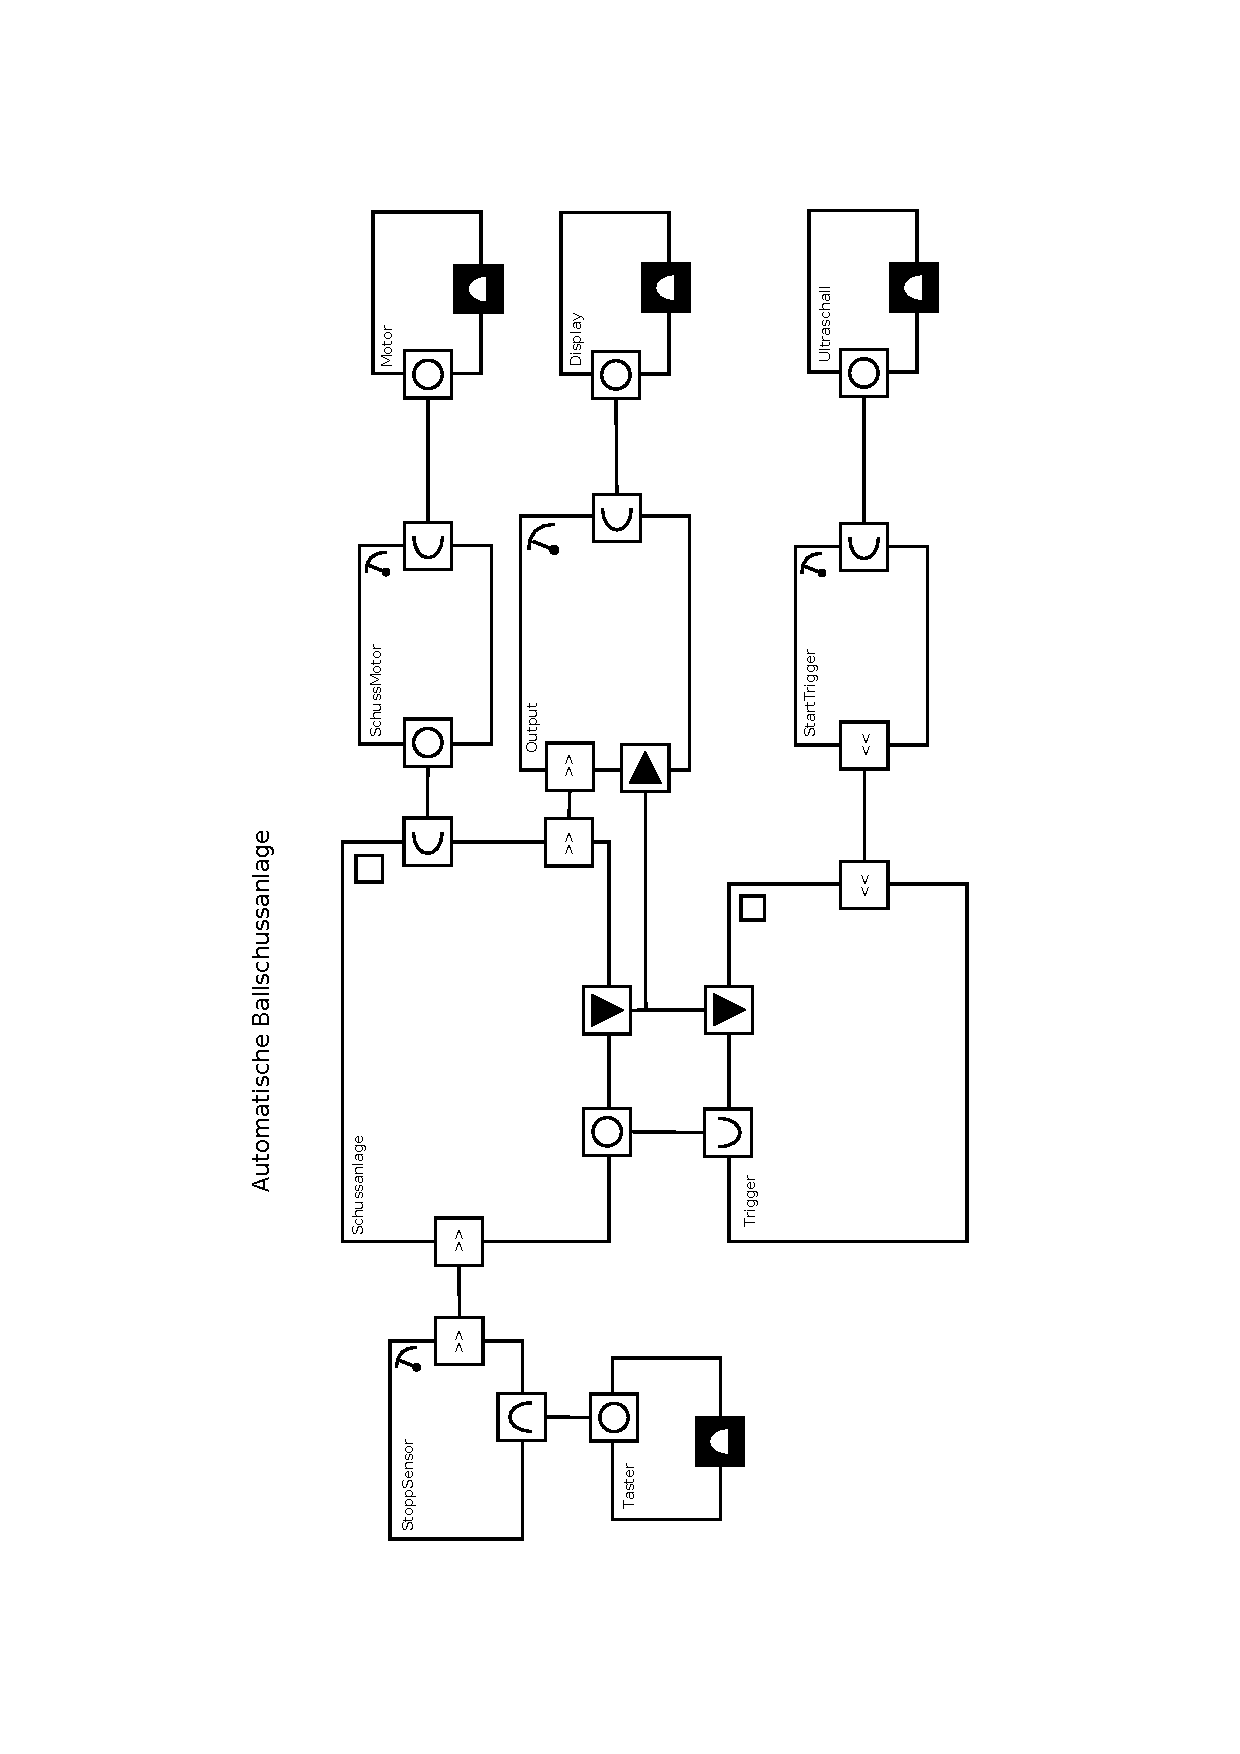
\includegraphics[scale=.75]{./KomponentenDiagramm.pdf}
 \label{fig:komponentendiag}
 \caption{Komponentendiagramm der Ballschussanlage (DT)}
\end{figure}

\section{Komponenten Funktionsapi}
Die Funktionsprototypen für die RTE-Funktionen sind in der Codedokumentation zu finden(unter \textit{YASA\_RTEAPI.h}).

\chapter{Komponenten-Beschreibung}

\section{Lose Beschreibung}

\subsection*{Schussanlage (FL)}

\begin{itemize}
	\item Besteht aus einer Task mit zwei Runnables
	\item erste Runnable prüft periodische die Abbruchbedinung(hier: Taster)
	\item zweite Runnable managt den Schussmotor
	\item Kein Autostart des Tasks, wird über den Trigger gestartet
	\item Ports siehe Komponentendiagramm
\end{itemize}

Benötigt: Task und Event

\subsection*{Trigger (PE)}

\begin{itemize}
 \item Ein Task
 \item Wird zu beginn gestartet (Autostart)
 \item Wartet auf Event vom Input
\end{itemize}

Benötigt: Task und Event

\subsection*{Output (MW)}

\begin{itemize}
 \item Autostart
 \item Wird durch Event von Schussanlage getriggert
 \item Prüft nach Event die empfangene Nachricht
 \item Zeigt Nachricht in Abhängigkeit der empfangen Nachricht an
\end{itemize}

Benötigt: Task und Event


\subsection*{SchussMotor (TimS)}

\begin{itemize}
 \item Kein Autostart
 \item Servertask wird durch Schussanlage (client) gestartet
 \item Steuert Motor zum schießen an
\end{itemize}


\subsection*{StopSensor (TobiS)}

\begin{itemize}
 \item Autostart
 \item Prüft Taster
 \item Setzt Event für Schussanlage
\end{itemize}

Benötigt: Task, Timer und Event


\subsection*{StartTrigger (TobiS)}

\begin{itemize}
 \item Task zum Erkennen von Zielen
 \item Autostart
 \item Sendet Event an Trigger
 \item Erkennung durch periodische Abfrage
\end{itemize}

Benötigt: Task und Timer

\section{Architekturschicht und Funktionsapi}

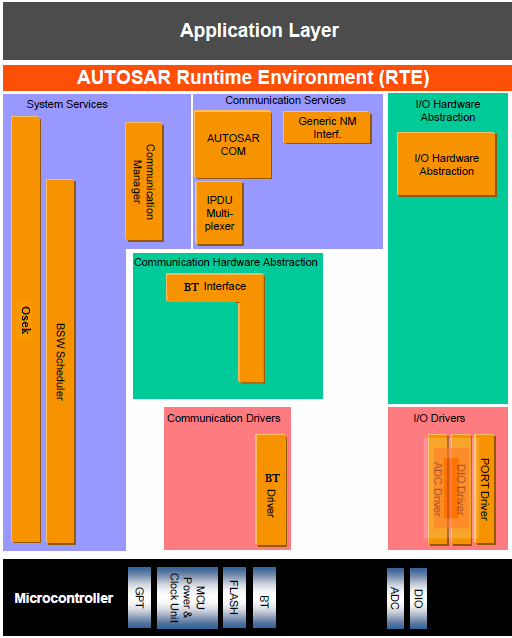
\includegraphics{Komponenten.png}

\subsection{Funktionapi}
\begin{enumerate}[1.)]
\item System Services\\
	keine Funktionen
\item Communication Services
	\begin{itemize}
	\item \underline{Abstraktionsebene um Nachrichten zu verschicken}
	\item \lstinline|StdReturnType TransmitMessage(char* message)|
	\item \lstinline|StdReturnType ReceiveMessage(char* message)|
	\end{itemize}
\item I/O Hardware Abstraction
	\begin{itemize}
	\item \lstinline|StdReturnType ReadDigitalInput(PortName)|
	\item \lstinline|StdReturnType ReadAnalogInput(PortName)|
	\item \lstinline|StdReturnType DriveMotor(Port_Name, Direction, speed, angle)|
	\end{itemize}
\item Communication Hardware Abstraction
	\begin{itemize}
	\item \underline{Für unser Projekt eigentlich unnötig, da wir nur eine Kommunikationsebene haben}(theoretisch mehr durch I2C, aber hier uninteressant)
	\item \lstinline|StdReturnType SendMessageBT(char* message )|
	\item \lstinline|StdReturnType GetMessageBT(char* message)|
	\end{itemize}
\item Communication Drivers
	\begin{itemize}
	\item \underline{es wird nur ein Treiber für das Hardware BT gebraucht:}
	\item \lstinline|StdReturnType BT_Write(char* message)| 
	\item \lstinline|StdReturnType BT_Read(char* message)|
	\end{itemize}
\item I/O Drivers
	\begin{itemize}
	\item \underline{benötigt für den zusätzlichen I2C expander}
	\item \lstinline|StdReturnType ReadI2C(PortName)|
	\item \lstinline|StdReturnType WriteI2C(PortName)|	
	\end{itemize}
\end{enumerate}

\section{Versendete Nachrichten}
Jede versendete Nachricht besteht aus 
\begin{itemize}
\item 1 Byte Header
\item bis zu 127 Byte Nachricht(allerdings mit terminierender $0$, das heißt nur 126 Byte Nutzdaten)
\end{itemize}
Diese Größe ist Applikationsspezifisch. Außerdem gibt es noch für jede Nachricht eine eindeutige \textit{ID}, diese wird allerdings nicht von der Applikation, sondern von den \textit{Communication Services} vergeben und versendet, bleibt also für die Applikation unsichtbar.
(TODO:)
2 Möglichkeiten: 1 Möglichkeit die der Nachrichtenheader wird auch im ComService aufgelöst und dann kann man nur noch die eigentlichen Daten an den entsprechenden Port weiterleiten oder aber der Header wird in der Applikation aufgelöst. Ich beschreibe hier Möglichkeit 2, dann sollte das System flexibler sein, das auflösen wird dann in der SW-Komponente über einen Funktionsaufruf gemacht
(End TODO)
\subsection{Nachricht}
Es gibt mehrere verschiedene Modi für Nachrichten:
\begin{enumerate}[1.)]
\item Nachricht: eine String-Nachricht soll übertragen:\\
	Nachrichtenheader $\&0x80 == 1 \Rightarrow$ zeigt das die folgende Nachricht einem String entspricht: Die restlichen Bits des Header zeigen an wie viele der folgenden Nachrichtenbytes gültig sind. Der Nachrichtenheader $\&0x7F$ zeigt an wie viele Bytes als Nachricht gültig sind.
\item Nachricht wird als Integer übertragen:
	Nachrichtenheader $\&0x80 == 0 \Rightarrow$ zeigt an das folgende Nachricht ein Integer sein muss. Dieser ist IMMER ein \textit{unsignend integer}. Es gilt weiterhin: Alle restlichen Bits des Nachrichtenheader \textbf{müssen} $0$ sein. Die folgende Nachricht muss ausserdem auch nur aus $0$en bestehen.
\item Nachricht wird als Event übertragen:
	Nachrichtenheader $\&0x80 == 0 \Rightarrow$ zeigt an das folgende Nachricht ein Event übertragen wird, wenn der Nachrichtenheader nicht aus lauter $0$en besteht. Dabei ist die Eventnummer die Zahl nach dem Nachrichtenheader $\&0x7F$. Es gibt als maximal 127 verschiedene Events. Die eigentliche Nachricht besteht nur aus $0$en.
\end{enumerate}
\subsection{Nachrichten-IDs}
Jede mögliche Nachricht hat eine eindeutige ID, diese wird von dem \textit{Com-Service} vergeben. Die Anzahl der IDs ist abhängig von der Applikation.\\ OS-spezifische Zugriffe können nicht über BT versendet werden und brauchen deswegen keine ID.
Folgende IDs sind für unsere Applikation vergeben:\\~\\
\centering
	\begin{tabular}{|c|c|c|}
	\hline
	\textbf{Verbindung} & \textbf{Porttyp} & \textbf{ID}\\
	\hline
	SAK StopSensor - SWK Schussanlage & Event & 1\\
	SWK Schussanlage - SAK Schussmotor & SenderReceiver & 2\\
	SAK Start\_Trigger - SWK Trigger & Event & 4\\
	SWK Schussanlage - SAK Output & Event & 8\\
	SWK Schussanlage - (SWK Trigger, SAK Output) & ServerClient & 16\\
	SWK Trigger - SWK Schussanlage & SenderReceiver & 32\\
	\hline
	\end{tabular}

\chapter{Konventionen/Definitionen}
hier werden alle Events,Tasks, Definitionen beschrieben, die immer implizit erfolgen
\section{Tasks}
\begin{itemize}
\item \lstinline|BT_IMPLIZIT_MASTER| Task der den Master im Bluetooth Verbund darstellt, den Verbindungsaufbau implementiert und senden und empfangen implementiert - Communication Driver
\item \lstinline|BT_IMPLIZIT_SLAVE| Task der den Slave im Bluetooth Verbund - Communication Driver
\item \lstinline|TASK_BT_INTERFACE| Task der die zu sendende/empfangende Nachricht erhält, das ganze parst(entweder zu string um zu versenden oder zurück wenn empfangen wurde) und eine ID hinzufügt
\end{itemize}
\section{globale Variablen}
\section{Events} 
für jede RTE-Funktion gibt es ein generiertes, von der Konfiguration abhängiges \lstinline|#define|. Der Namensaufbau ist definiert durch
\lstinline|Funktionsname_(ONEBRICK,TWOBRICK,THREEBRICK)|. Dabei muss in der Konfiguration das jeweilige Makro gesetzt werden, wobei
\begin{itemize}
\item \lstinline|ONEBRICK| die Verbindung der beteiligten Bricks liegt auf einem Brick
\item \lstinline|TWOBRICK| die Verbindung der beteiligten Bricks liegen auf unterschiedlichen Bricks
\item \lstinline|THREEBRICK| mind. eine Verbindung liegt auf einem Brick und mind. eine Verbindung liegt auf einem anderen Brick(geht natürlich nur bei Multicast).
\end{itemize}


\end{document}

